\section{Package client}
In questa sezione verranno descritti il package \texttt{client} e le classi che lo compongono.\\

\subsection{Main}
La classe \texttt{Main} è il punto di ingresso dell'applicazione client.
Essa si occupa di inizializzare il modello principale (\texttt{MainModel}) e di lanciare l'interfaccia grafica utente \texttt(GUI).
Il metodo \texttt{main} avvia l'applicazione creando un'istanza di \texttt{Main} e chiamando il metodo \texttt{launchGUI}.\\
I metodi di tale classe sono:
\begin{itemize}
    \item \texttt{public void launchGUI()}: fa partire l'interfaccia grafica dell'appplicazione.
    \item \texttt{public static void main(String[] args)}: metodo di ingresso dell'applicazione.
\end{itemize}

\subsection{Package models}
In questa sezione verranno descritti il package \texttt{models} e le classi che lo compongono.\\

\subsubsection{CurrentOperator}
La classe \texttt{CurrentOperator} è un singleton che gestisce lo stato dell'operatore attualmente loggato.
Fornisce metodi per settare e recuperare l'operatore corrente, controllare lo stato di login, effettuare il logout e gestire i listener che osservano i cambiamenti dell'operatore corrente.
Questa classe usa il pattern Singleton per assicurarsi che ci sia una sola istanza di \texttt{CurrentOperator}.
I metodi di tale classe sono:
\begin{itemize}
    \item \texttt{public static CurrentOperator getInstance()}: restituisce l'istanza corrente di \texttt{CurrentOperator}.
    \item \texttt{public void setCurrentOperator(RecordOperator operator)}: imposta l'operatore corrente.
    \item \texttt{public RecordOperator getCurrentOperator()}: restituisce l'operatore attualmente loggato.
    \item \texttt{public boolean isUserLogged()}: controlla se l'operatore corrente è loggato.
    \item \texttt{public void performLogout()}: setta l'operatore corrente a null.
    \item \texttt{void onCurrentUserChange(RecordOperator newOperator)}: metodo chiamato quando l'operatore corrente cambia.
    \item \texttt{public void addCurrentUserChangeListener(CurrentUserChangeListener listener)}: aggiunge un listener per osservare i cambiamenti dell'operatore corrente.
    \item \texttt{public void removeCurrentUserChangeListener(CurrentUserChangeListener listener)}: rimuove un listener dalla lista di osservatori.
    \item \texttt{private void notifyCurrentUserChange()}: notifica tutti i listener registrati che l'operatore corrente è cambiato.
\end{itemize}

\subsubsection{MainModel}
La classe \texttt{MainModel} è responsabile della connessione ai servizi RMI (Remote Method Invocation) e del recupero delle interfacce remote. Queste interfacce permettono al client di comunicare con il server ed eseguire operazioni remote come la gestione dei dati, le query sui dati e la logica operativa.
Il costruttore della classe si occupa di localizzare il registro RMI e di effettuare il lookup delle interfacce remote. In caso di errore durante il processo di lookup, viene lanciata una RuntimeException.

\begin{figure}[H]
    \centering
    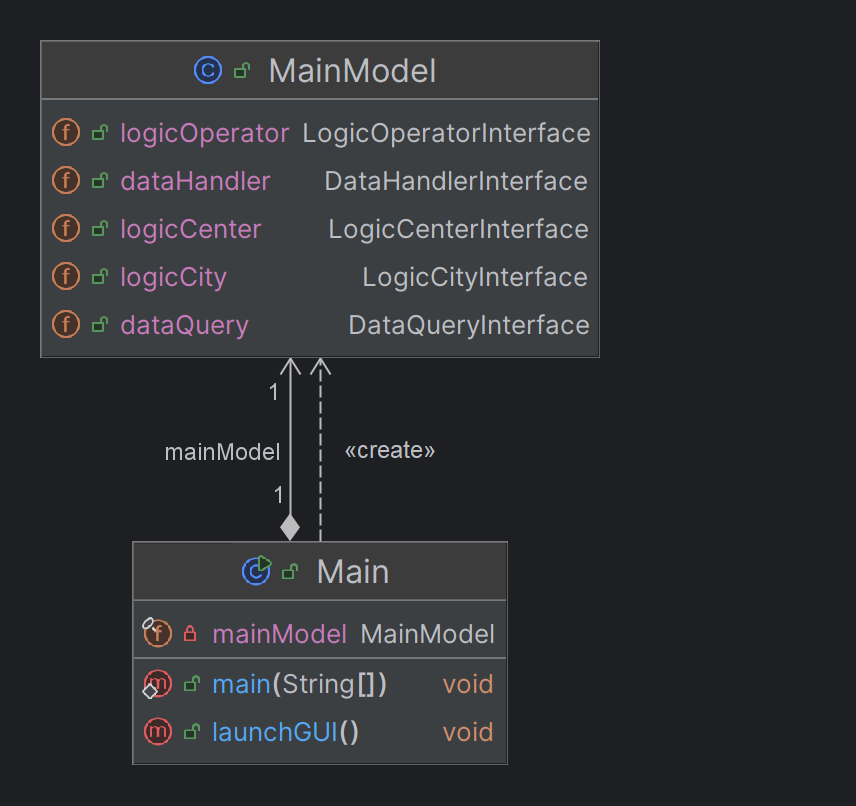
\includegraphics[width=0.7\textwidth]{img/mainModelUML.png}
    \caption{UML della classe MainModel}
    \label{fig:UMLMainModel}
\end{figure}
Oltre aigli attributi è presente solo un costruttore:
\begin{itemize}
    \item \texttt{public MainModel()}: ottiene il registro RMI creato dal server e cerca le interfacce remote necessarie per la comunicazione con lo stesso.
\end{itemize}

\subsection{Package GUI}
In questa sezione verranno descritti il package \texttt{GUI} e le classi che lo compongono.\\

\begin{figure}[H]
    \centering
    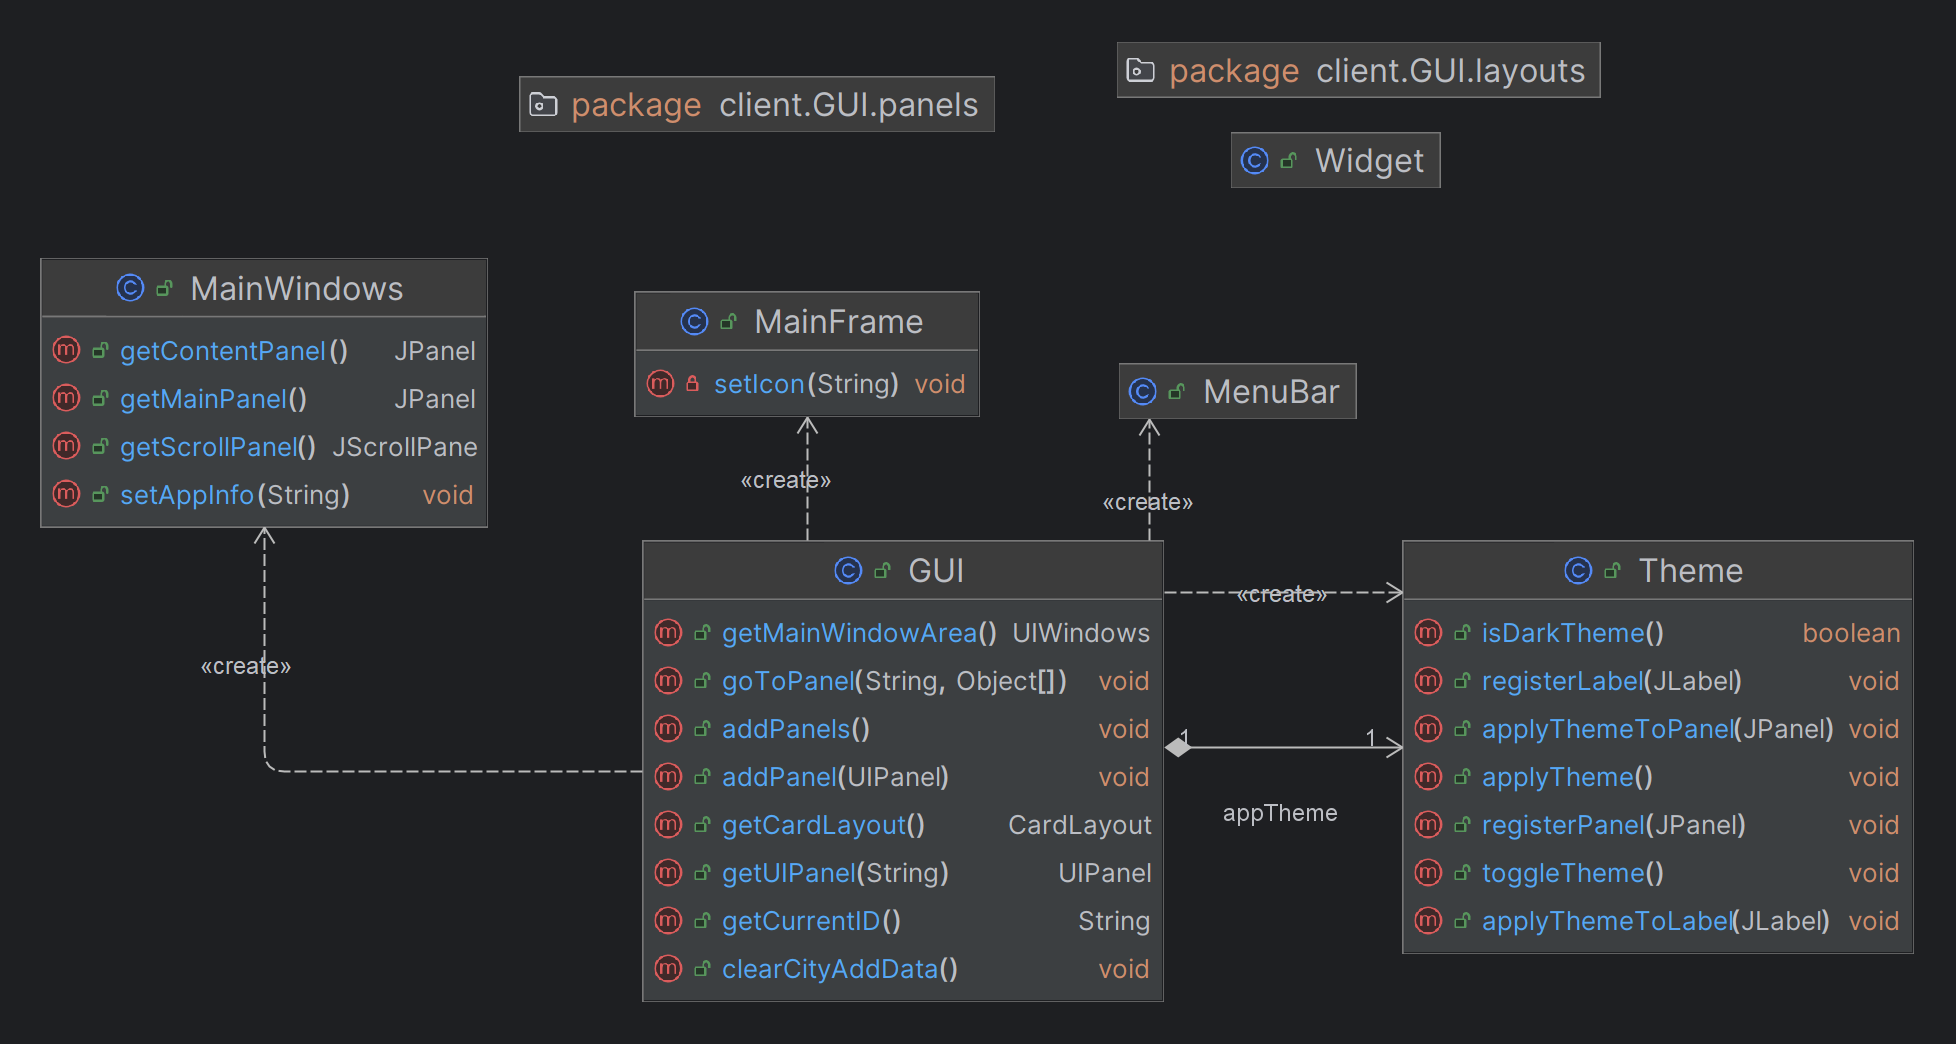
\includegraphics[width=0.9\textwidth]{img/guiPackage.png}
    \caption{UML del package GUI}
    \label{fig:UMLGUI} 
\end{figure}

\subsubsection {GUI}
La classe \texttt{GUI} gestisce l'interfaccia utente dell'applicazione e la navigazione tra diversi pannelli. 
È una componente chiave dell'architettura dell'applicazione, responsabile della creazione e gestione dei pannelli dell'interfaccia utente e della loro visualizzazione.
I metodi di tale classe sono:
\begin{itemize}
    \item \texttt{public void addPanels()}: aggiunge tutti i pannelli utilizzati nell'applicazione.
    \item \texttt{public void addPanel(Interfaces.UIPanel Panel)}: aggiunge un pannello alla mappa dei pannelli e gli applica il tema grafico.
    \item \texttt{public void clearCityAddData()}: pulisce i dati inseriti nel pannello di aggiunta dati di una città.
    \item \texttt{public Interfaces.UIPanel getUIPanel(String ID)}: ottiene un pannello dell'interfaccia utente in base al suo ID.
    \item \texttt{public Interfaces.UIWindows getMainWindowArea()}: restituisce l'area principale dell'applicazione.
    \item \texttt{public CardLayout getCardLayout()}: restituisce il layout a schede utilizzato per la navigazione tra i pannelli.
    \item \texttt{public String getCurrentID()}: restituisce l'ID del pannello corrente.
    \item \texttt{public void goToPanel(String ID, Object[] args)}: cambia il pannello corrente in base all'ID specificato.
\end{itemize}

\subsubsection {Theme}
La classe \texttt{Theme} gestisce il tema grafico dell'applicazione, inclusa la modalitàchiaro/scuro, e applica il tema alle etichette ({@code JLabel}) e ai pannelli ({@code JPanel}).
La classe consente di passare tra modalità chiara e scura e applica automaticamente il tema corrente a tutti i componenti registrati.
I metodi di tale classe sono:
\begin{itemize}
    \item \texttt{public void toggleTheme()}: passa tra modalità chiara e scura.
    \item \texttt{public boolean isDarkTheme()}: controlla se il tema corrente è scuro.
    \item \texttt{public void registerLabel(JLabel label)}: registra un'etichetta per applicare il tema corrente.
    \item \texttt{public void registerPanel(JPanel panel)}: registra un pannello per applicare il tema corrente.
    \item \texttt{public void applyTheme()}: applica il tema corrente a tutti i componenti registrati.
    \item \texttt{public void applyThemeToPanel(JPanel panel)}: applica il tema corrente a un pannello.
    \item \texttt{public void applyThemeToLabel(JLabel label)}: applica il tema corrente a un'etichetta.
\end{itemize}

\subsubsection {Widget}
La classe \texttt{Widget} fornisce componenti grafici comuni utilizzati nell'interfaccia utente dell'applicazione tramite classi interne.\\
Include pannelli di formattazione, pulsanti con cursori personalizzati, etichette per immagini e oggetti per elementi di una lista a discesa. 
Questi componenti sono progettati per facilitare la creazione di interfacce utente coerenti e ben stilizzate.

\begin{figure}[H]
    \centering
    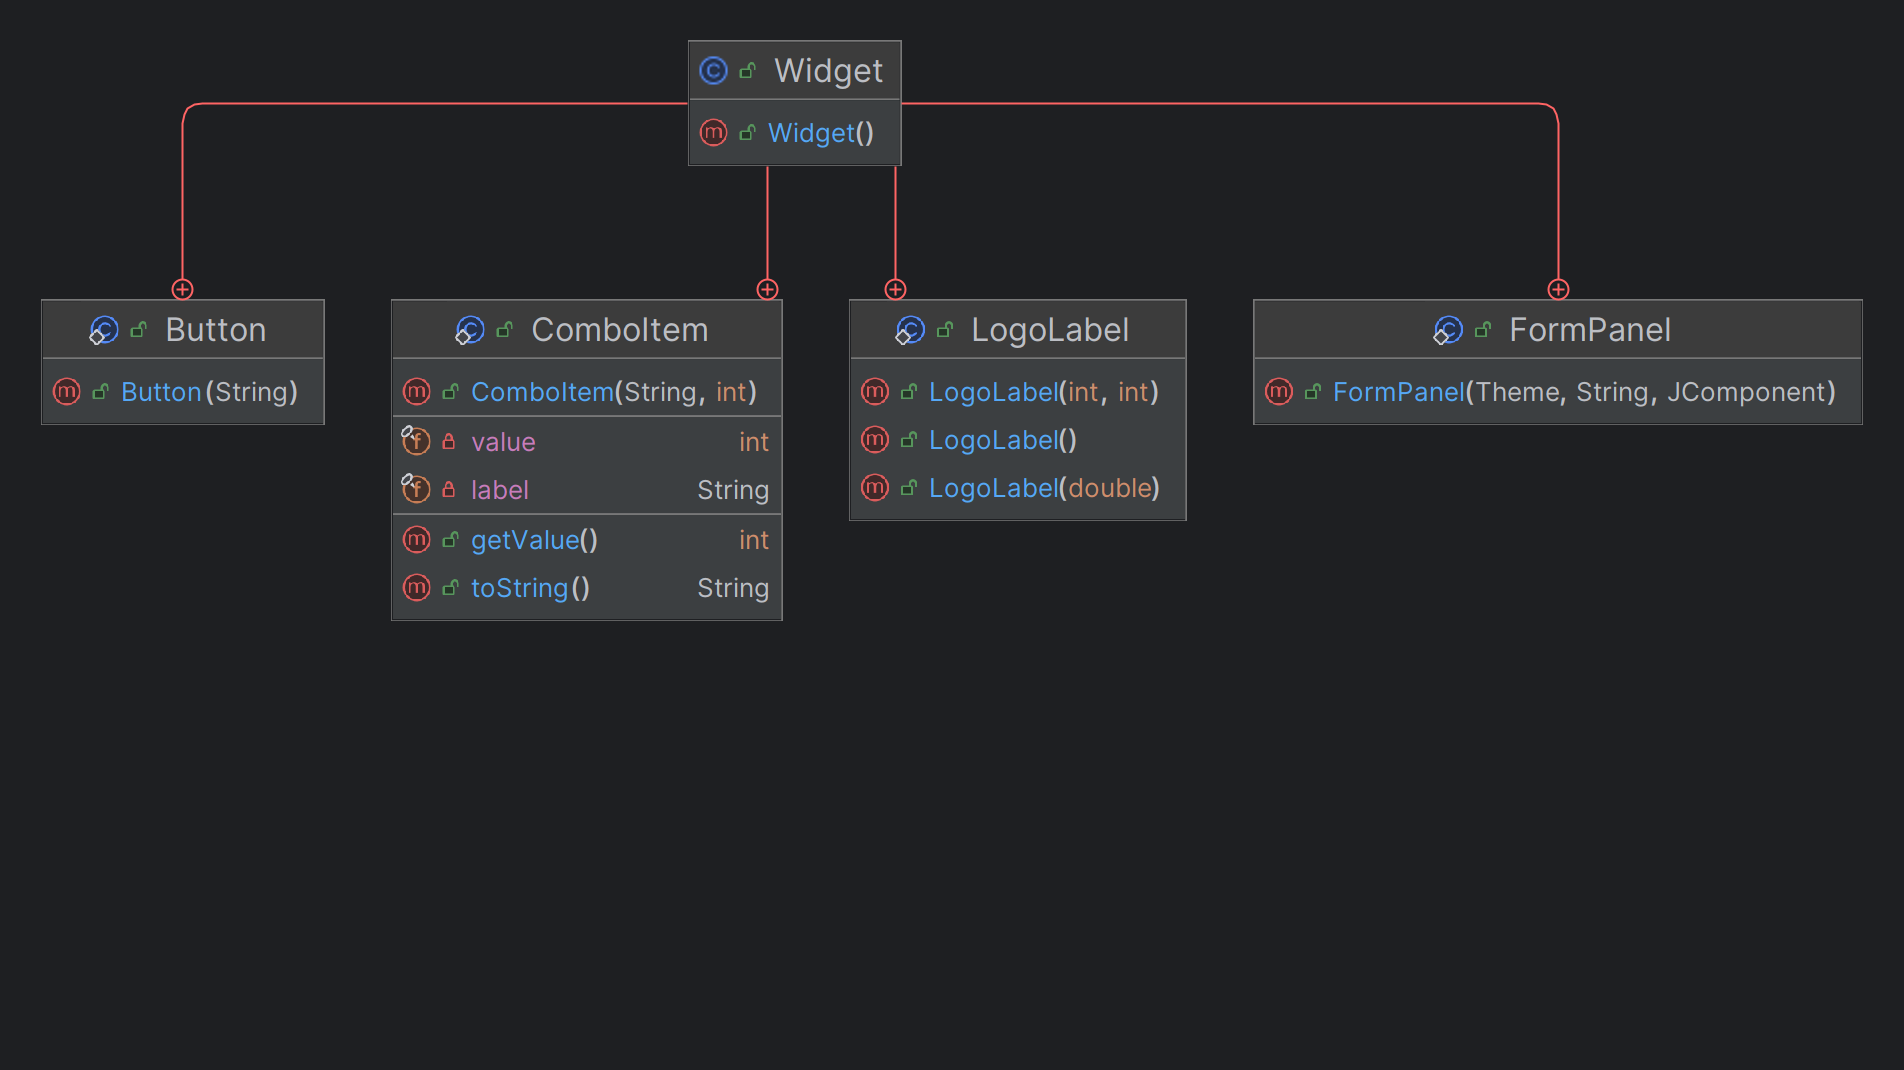
\includegraphics[width=0.9\textwidth]{img/UMLWidget.png}
    \caption{UML della classe Widget}
    \label{fig:UMLWidget}
\end{figure}
I costruttori e metodi delle classi interne sono:
\begin{itemize}
    \item \texttt{public FromPanel(Theme appTheme, String labelText, JComponent activeArea)}: costruttore del pannello di formattazione personalizzato.
    \item \texttt{public Button(String text)}: costruttore di un pulsante con il testo specificato.
    \item \texttt{public LogoLabel()}: crea un'etichetta con le dimensioni predefinite.
    \item \texttt{public LogoLabel(double scale)}: crea un'etichetta con le dimensioni specificate per il logo.
    \item \texttt{public LogoLabel(int width, int height)}: crea un'etichetta dimensioni personalizzate.
    \item \texttt{public ComboItem(String label, int value)}: costruttore di un oggetto per un elemento di una lista a discesa con un'etichetta e un valore associato.
    \item \texttt{public int getValue()}: restituisce il valore associato all'elemento della lista a discesa.
    \item \texttt{public String toString()}: restituisce l'etichetta dell'elemento della lista a discesa.
\end{itemize}

\subsubsection{Package layouts}
In questo package sono presenti le classi che definiscono i layout utilizzati nell'interfaccia grafica dell'applicazione.

\begin{figure}[H]
    \centering
    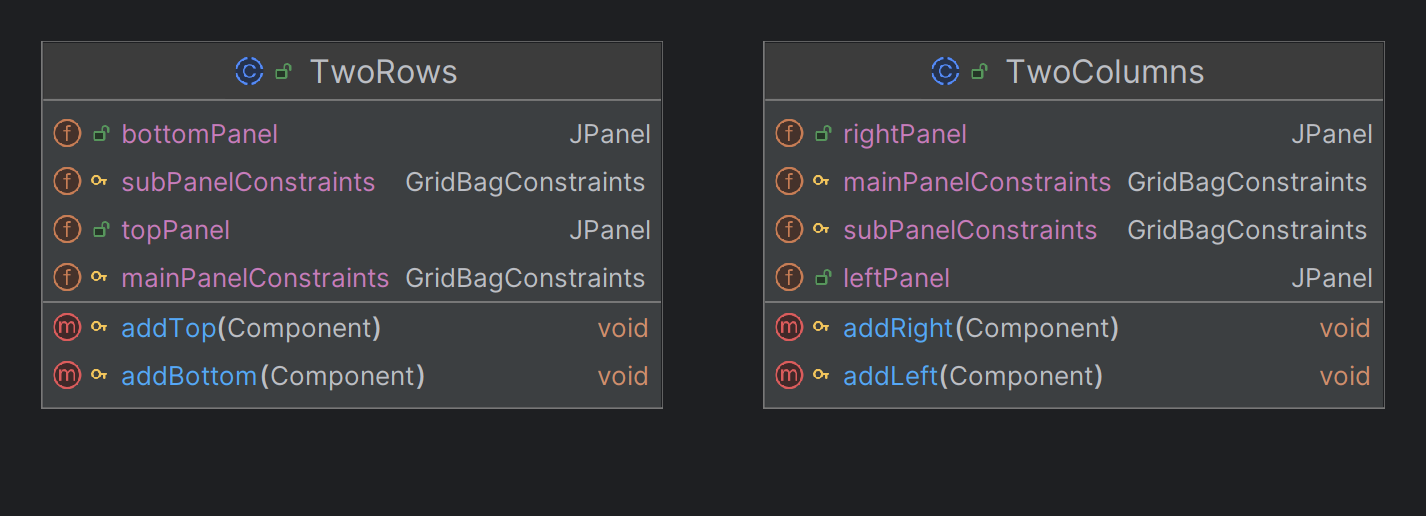
\includegraphics[width=0.9\textwidth]{img/layoutsPackage.png}
    \caption{UML del package layouts}
    \label{fig:UMLLayouts}
\end{figure}
\paragraph{TwoColumns}
La classe astratta \texttt{TwoColumns} rappresenta un layout a due colonne, con un pannello sinistro e un pannello destro. È progettata per essere estesa da altre classi che necessitano di questo tipo di layout.
Entrambi i pannelli utilizzano un \texttt{GridBagLayout} per permettere un layout flessibile dei componenti.
La classe fornisce metodi protetti per aggiungere componenti ai pannelli sinistro e destro.\\
I metodi di tale classe sono:
\begin{itemize}
    \item \texttt{protected void addLeft(Component component)}: aggiunge un componente al pannello sinistro.
    \item \texttt{protected void addRight(Component component)}: aggiunge un componente al pannello destro.
\end{itemize}

\paragraph{TwoRows}
La classe astratta \texttt{TwoRows} rappresenta un layout a due righe per un'interfaccia grafica Swing.
Le due righe contengono un pannello superiore e un pannello inferiore per organizzare i componenti dell'interfaccia.\\
I metodi di tale classe sono:
\begin{itemize}
    \item \texttt{protected void addTop(Component component)}: aggiunge un componente al pannello superiore.
    \item \texttt{protected void addBottom(Component component)}: aggiunge un componente al pannello inferiore.
\end{itemize}

\subsubsection {Package mainElements}
In questo package sono presenti le classi che definiscono gli elementi della finestra principale dell'applicazione.

\begin{figure}[H]
    \centering
    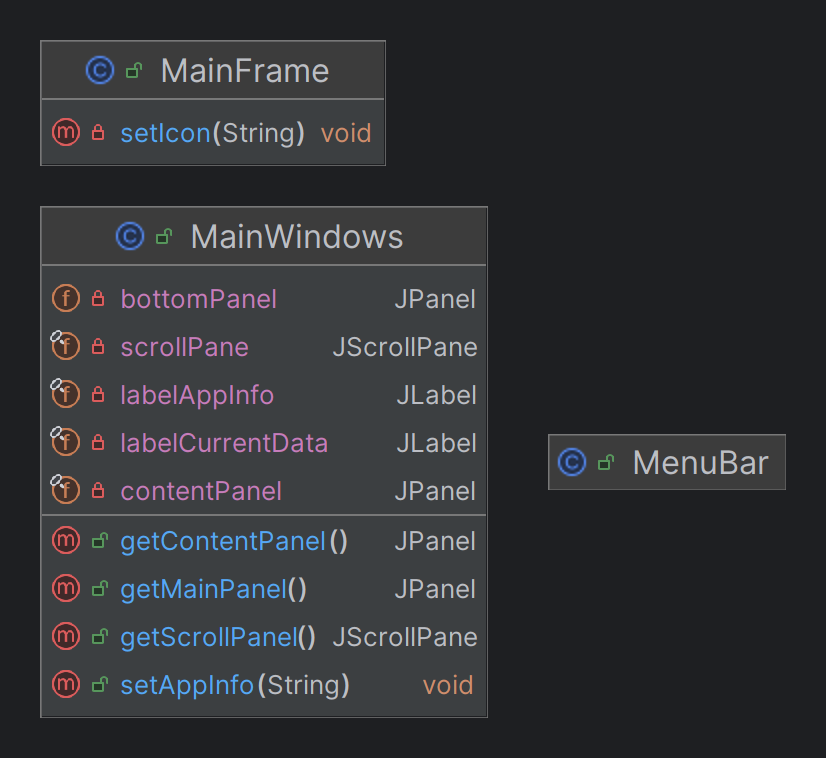
\includegraphics[width=0.6\textwidth]{img/mainElementsPackage.png}
    \caption{UML del package mainElements}
    \label{fig:UMLMainElements}
\end{figure}

\paragraph{MainFrame}
La classe \texttt{MainFrame} rappresenta il frame principale dell'applicazione.
Il frame contiene i componenti principali dell'interfaccia utente e funge da contenitore principale per tutti i widget e pannelli dell'applicazione.
I costruttori e metodi di tale classe sono:
\begin{itemize}
    \item \texttt{public MainFrame()}: configura il frame principale dell'applicazione.
    \item \texttt{private void setIcon(String iconPath)}: imposta l'icona del frame.
\end{itemize}

\paragraph{MainWindows}
La classe \texttt{MainWindows} rappresenta la finestra principale dell'applicazione.
Questa finestra contiene un pannello scorrevole con un layout a schede, in cui vengono visualizzate diverse schermate dell'applicazione. 
Inoltre, nella parte inferiore della finestra, vengono visualizzate informazioni sull'operatore attualmente loggato e l'orario corrente.
I costruttori e metodi di tale classe sono:
\begin{itemize}
    \item \texttt{public MainWindows(CardLayout cardLayout)}: inizializza la finestra principale dell'applicazione impostando il pannello a scorrimento, il layout a schede e aggiungendo timer e informazioni sull'operatore nella parte inferiore della finestra.
    \item \texttt{public JPanel getMainPanel()}: restituisce il pannello principale della finestra.
    \item \texttt{public JScrollPane getScrollPanel()}: restituisce il pannello scorrevole della finestra.
    \item \texttt{public JPanel getContentPanel()}: restituisce il pannello contenente i pannelli a schede.
    \item \texttt{public void setAppInfo(String text)}: imposta le informazioni sull'operatore attualmente loggato.
\end{itemize}

\paragraph{MenuBar}

La classe \texttt{MenuBar} rappresenta la barra del menù dell'interfaccia grafica dell'applicazione.
Questa barra del menù consente la navigazione tra diverse sezioni dell'applicazione e fornisce opzioni per cambiare il tema dell'interfaccia utente e gestire la sessione dell'operatore.
Gli elementi principali del menù includono home, ricerca città, e un sotto-menù per l'area operatore con le opzioni di login, registrazione, gestione città e logout.
All'interno è presente solo il costruttore:
\begin{itemize}
    \item \texttt{public MenuBar(GUI gui)}: imposta il layout della barra del menu, aggiunge gli elementi del menu e gestisce gli eventi di selezione del menu.
\end{itemize}

\subsubsection {Package panels}
In questo package sono presenti le classi che definiscono i pannelli dell'interfaccia grafica dell'applicazione.

\begin{figure}[H]
    \centering
    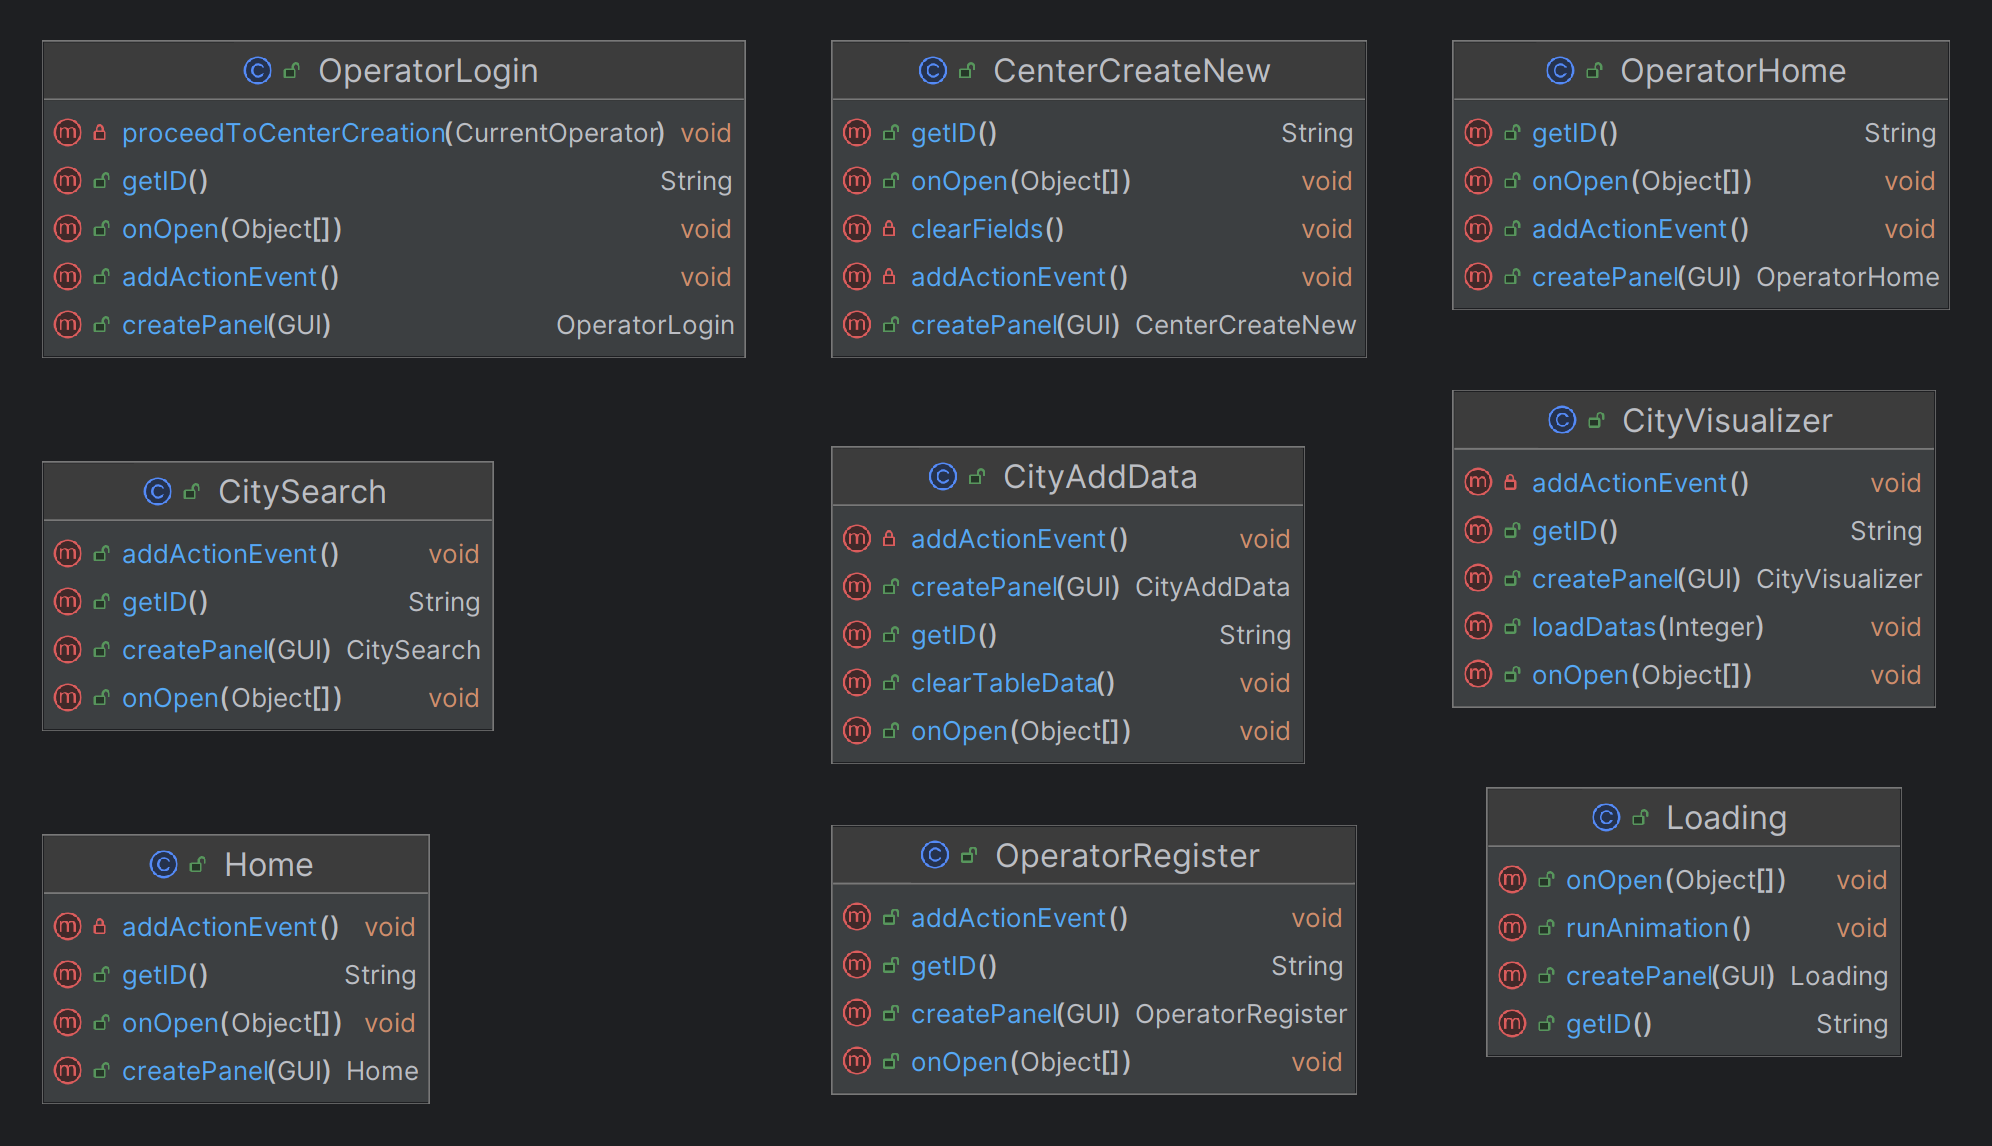
\includegraphics[width=0.9\textwidth]{img/panelsPackage.png}
    \caption{UML del package panels}
    \label{fig:UMLPanels}    
\end{figure}

\paragraph{Loading}
La classe \texttt{Loading} rappresenta un pannello di caricamento animato che viene visualizzato all'avvio dell'applicazione.
Questo pannello mostra il nome dell'applicazione con una serie di punti che si muovono per simulare un caricamento. 
L'animazione prosegue fino a quando il pannello non reindirizza automaticamente all'homepage dell'applicazione.
I metodi di tale classe sono:
\begin{itemize}
    \item \texttt{public void runAnimation()}: avvia l'animazione di caricamento.
    \item \texttt{public Loading createPanel(GUI gui)}: crea il pannello di caricamento.
    \item \texttt{public String getID()}: restituisce l'ID del pannello.
    \item \texttt{public void onOpen(Object[] args)}; gestisce l'apertura del pannello.
\end{itemize}

\paragraph{Home}
La classe \texttt{Home} rappresenta il pannello principale dell'applicazione visualizzato dopo il caricamento iniziale.
Questo pannello fornisce all'utente due opzioni principali: \textbf{Cerca e visualizza dati} per accedere alla funzionalità di ricerca e visualizzazione dei dati, e \textbf{Gestisci area operatore} per accedere alla gestione dell'area riservata agli operatori.
L'utente può selezionare una delle opzioni per avviare le funzionalità specifiche dell'applicazione.
I metodi di tale classe sono:
\begin{itemize}
    \item \texttt{private void addActionEvent()}: aggiunge gli eventi per la navigazione tra i pannelli.
    \item \texttt{public Home createPanel(GUI gui)}: crea il pannello home.
    \item \texttt{public String getID()}: restituisce l'ID del pannello.
    \item \texttt{public void onOpen(Object[] args)}: gestisce l'apertura del pannello.
\end{itemize}

\paragraph{CitySearch}
La classe \texttt{CitySearch} rappresenta il pannello  per effettuare ricerche sulla base di dati delle città.
Gli utenti possono cercare una città per nome o per coordinate geografiche utilizzando i campi di input e i pulsanti forniti.
I metodi di tale classe sono:
\begin{itemize}
    \item \texttt{public void addActionEvent()}: aggiunge gli eventi per la ricerca delle città in base al pulsante premuto.
    \item \texttt{public CitySerch createPanel(GUI gui)}: crea il pannello di ricerca città.
    \item \texttt{public String getID()}: restituisce l'ID del pannello.
    \item \texttt{public void onOpen(Object[] args)}: gestisce l'apertura del pannello.
\end{itemize}

\paragraph{CityVisualizer}

La classe \texttt{CityVisualizer} rappresenta il pannello per la visualizzazione dei dati di una città, inclusi i dati meteorologici relativi a diverse categorie.
È utilizzato nell'applicazione per mostrare dettagli sulla città selezionata e i dati meteorologici associati.
I metodi di tale classe sono:
\begin{itemize}
    \item \texttt{private void addActionEvent()}: aggiunge gli eventi al pulsante per tornare alla schermata precedente.
    \item \texttt{public void loadDatas(Integer cityID)}: carica i dati della città selezionata.
    \item \texttt{public CityVisualizer createPanel(GUI gui)}: crea il pannello di visualizzazione dei dati della città.
    \item \texttt{public String getID()}: restituisce l'ID del pannello.
    \item \texttt{public void onOpen(Object[] args)}: gestisce l'apertura del pannello.
\end{itemize}
Sono presenti anche due classi interne:
\begin{itemize}
    \item \texttt{ToolttipCellRenderer}: classe interna che gestisce il rendering delle celle della tabella.
    \item \texttt{NonEditableCellEditor}: classe interna per l'editor delle celle non modificabili.
\end{itemize}

\begin{figure}[H]
    \centering
    \includegraphics[width=0.9\textwidth]{img/cityVisualizerUML.png}
    \caption{UML della classe CityVisualizer}
    \label{fig:UMLCityVisualizer}
\end{figure}

I metodi di tali classi interne sono:
\begin{itemize}
    \item \texttt{public Component getTableCellRendererComponent(JTable table, Object value, boolean isSelected, boolean hasFocus, int row, int column)}: restituisce il componente per il rendering delle celle della tabella.
    \item \texttt{public boolean isCellEditable(EventObject e)}: restituisce \texttt{false} per indicare che la cella non è modificabile.
\end{itemize}

\paragraph{OperatorHome}
La classe \texttt{OperatorHome} rappresenta il pannello principale per gli operatori dell'applicazione.
Da questo pannello, gli operatori possono scegliere di registrarsi o accedere all'applicazione. 
Questa classe gestisce la navigazione tra il pannello di registrazione e quello di login tramite i pulsanti corrispondenti.
I metodi di tale classe sono:
\begin{itemize}
    \item \texttt{public void addActionEvent()}: aggiunge gli eventi per la navigazione tra i pannelli in base al pulsante premuto.
    \item \texttt{public String getID()}: restituisce l'ID del pannello.
    \item \texttt{public void onOpen(Object[] args)}: gestisce l'apertura del pannello.
\end{itemize}

\paragraph{OperatorRegister}
La classe \texttt{OperatorRegister} rappresenta il pannello utilizzato per la registrazione di un operatore all'interno dell'applicazione.
Questo pannello consente agli operatori di inserire i loro dati personali, come nome, codice fiscale, email, username e password, al fine di creare un nuovo account operatore.
Utilizza il modulo server RMI per la registrazione e gestisce le eccezioni che possono derivare dalla connessione al server o dalle operazioni sul database.
I metodi di tale classe sono:
\begin{itemize}
    \item \texttt{public void addActionEvent()}: aggiunge gli eventi per la registrazione dell'operatore.
    \item \texttt{public OperatorRegister createPanel(GUI gui)}: crea il pannello di registrazione operatore.
    \item \texttt{public String getID()}: restituisce l'ID del pannello.
    \item \texttt{public void onOpen(Object[] args)}: gestisce l'apertura del pannello.
\end{itemize}

\paragraph{OperatorLogin}
La classe \texttt{OperatorLogin} rappresenta il pannello di login per gli operatori dell'applicazione.
Gli operatori possono inserire il loro username e la password per accedere all'applicazione. 
Utilizza un modulo server RMI per autenticare l'operatore e interagisce con un database per recuperare e gestire i dati necessari.
I metodi di tale classe sono:
\begin{itemize}
    \item \texttt{public void addActionEvent()}: aggiunge gli eventi per il login dell'operatore.
    \item \texttt{public OperatorLogin createPanel(GUI gui)}: crea il pannello di login operatore.
    \item \texttt{public String getID()}: restituisce l'ID del pannello.
    \item \texttt{public void onOpen(Object[] args)}: gestisce l'apertura del pannello.
    \item \texttt{private void proceedToCenterCreation(CurrentOperator currentOperator)}: metodo privato che gestisce la creazione o associazione di un centro per l'operatore che ha effettuato il login per la prima volta.

\end{itemize}

\paragraph{CenterCreateNew}
La classe \texttt{CenterCreateNew} rappresenta il pannello per la creazione di un nuovo centro di monitoraggio da parte dell'operatore.
Il pannello consente all'operatore di inserire informazioni sul centro, come il nome, la via, il numero civico, il CAP, il comune, la provincia e le città associate al centro.\\
Una volta inseriti i dati, l'operatore può salvare il centro nel sistema utilizzando i servizi offerti dal modulo server RMI e interagendo con il database.\\
La classe gestisce la validazione dei dati inseriti e fornisce feedback all'operatore in caso di errori.\\
La comunicazione con il server RMI è gestita attraverso l'interfaccia \texttt{DataQueryImp} per le query sui dati e \texttt{MainModel} per la logica di applicazione.
I metodi di tale classe sono:
\begin{itemize}
    \item \texttt{private void clearFields()}: pulisce i campi di input del pannello.
    \item \texttt{private void addActionEvent()}: aggiunge gli eventi per la creazione di un nuovo centro.
    \item \texttt{public CenterCreateNew createPanel(GUI gui)}: crea il pannello di creazione di un nuovo centro.
    \item \texttt{public String getID()}: restituisce l'ID del pannello.
    \item \texttt{public void onOpen(Object[] args)}: gestisce l'apertura del pannello.
\end{itemize}

\paragraph{CityAddData}
La classe \texttt{CityAddData} rappresenta il pannello per l'aggiunta di dati di una città da parte dell'operatore.\\
Il pannello consente all'operatore di inserire i dati relativi alla città selezionata quali: data di rilevamento dati, punteggi per le varie categorie ed eventualmente dei commenti che li descrivono.\\
La classe gestisce la validazione della data inserita, il limite di caratteri per i commenti dei dati e la funzionalità per il salvataggio dei dati inseriti. 
I metodi di tale classe sono:
\begin{itemize}
    \item \texttt{public void clearTableData()}: pulisce i dati inseriti nella tabella.
    \item \texttt{private void addActionEvent()}: aggiunge gli eventi per l'aggiunta dei dati della città.
    \item \texttt{public CityAddData createPanel(GUI gui)}: crea il pannello di aggiunta dati di una città.
    \item \texttt{public String getID()}: restituisce l'ID del pannello.
    \item \texttt{public void onOpen(Object[] args)}: gestisce l'apertura del pannello.
\end{itemize}
Anche in questo caso sono presenti delle classi interne:
\begin{itemize}
    \item \texttt{IntegerCellEditor}: classe interna per l'editor delle celle numeriche.
    \item \texttt{ToolttipCellRenderer}: classe interna che gestisce il rendering delle celle della tabella.
    \item \texttt{NonEditableCellEditor}: classe interna per l'editor delle celle non modificabili.
\end{itemize}
I metodi di tali classi interne sono:
\begin{itemize}
    \item \texttt{public Integer getCellEditorValue()}: restituisce il valore intero selezionato dall'utente.
    \item \texttt{public Component getTableCellRendererComponent(JTable table, Object value, boolean isSelected, boolean hasFocus, int row, int column)}: restituisce il componente per il rendering delle celle della tabella.
    \item \texttt{public boolean isCellEditable(EventObject e)}: resituisce \texttt{false} per indicare che la cella non è modificabile.
\end{itemize}